We have established that there are pronounced gender differences in the patterns of positive and statistically significant treatment effects.\footnote{We summarize previous research on gender differences in Table~\ref{tab:litreview-table}.} Figure~\ref{fig:ppositive} reports the estimated combining functions by gender and by category of care used by the control group.\footnote{See Appendix~\ref{appendix:results} for estimates of individual treatment effects and additional specifications of combining functions.}

The null hypothesis  of no treatment effect is equivalent to the hypothesis that the proportion of outcomes is equal to $0.500$. Figure~\ref{fig:ppositivehome} displays combining functions for treatment effects comparing outcomes of the treated to outcomes for those who stay at home. Figure~\ref{fig:ppositivealternative} displays analogous combining functions comparing treatment effects of those participating in ABC/CARE to those who attend alternative formal childcare. These estimates account for selection into the mode of childcare using matching.

Comparing ABC/CARE to those who stay at home (Figure~\ref{fig:ppositivehome}), a greater proportion of the treatment effects is positive for women than for men. While the female proportion is statistically significantly larger than $0.500$, the male proportion is not. Figure~\ref{fig:ppositivealternative} shows a different pattern when we compare outcomes from ABC/CARE with outcomes of those who attended alternative formal childcare. Close to 75\% of the treatment effects are positive for men. For women, the proportion of positive treatment effects is similar to the proportion obtained by comparing ABC/CARE to those who stay at home. From this analysis, we conclude that ABC/CARE was effective for men compared to alternative formal childcare programs, but not when compared to staying at home. ABC/CARE was effective for women regardless of the mode of childcare used by the controls.\footnote{Disaggregating by outcomes, by category, gender, and mode of childcare for controls produces a noisy pattern that is broadly consistent in Figure~\ref{fig:ppositive}.}

\begin{sidewaysfigure}[!htbp]
\centering
\caption{Positively Impacted Outcomes, ABC/CARE Males and Females}\label{fig:ppositive}
\begin{subfigure}[h]{0.5\textwidth}
	\centering
	\caption{Treatment vs.\ Stay at Home} \label{fig:ppositivehome}
	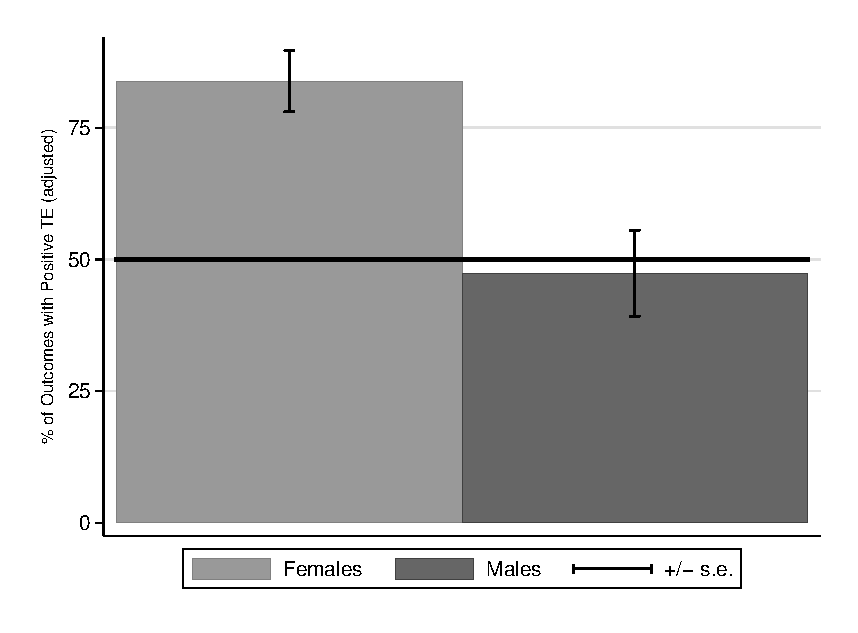
\includegraphics[width=\textwidth]{output/epan_ipw_p0_all.eps}
\end{subfigure}%
\begin{subfigure}[h]{0.5\textwidth}
	\centering
	\caption{Treatment vs.\ Alternative Formal Childcare} \label{fig:ppositivealternative}
		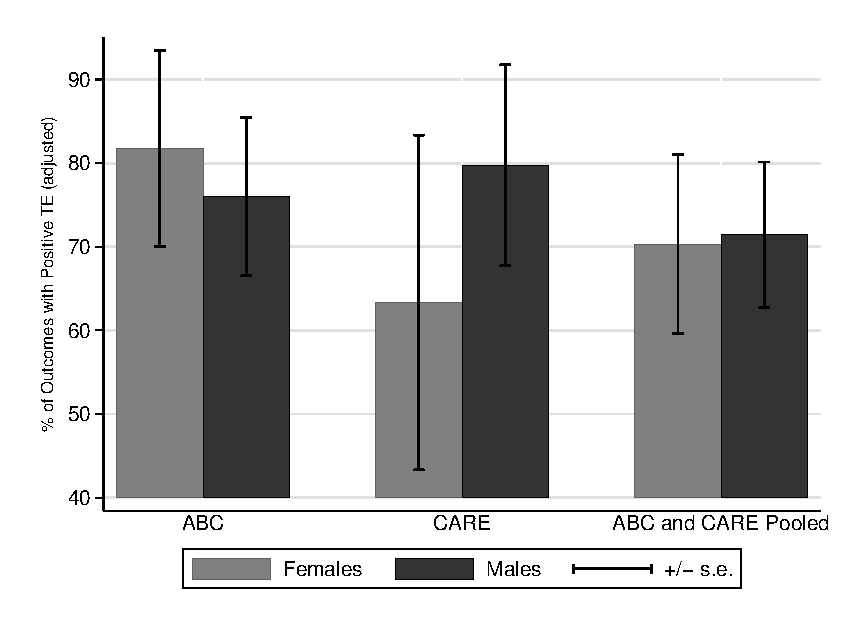
\includegraphics[width=\textwidth]{output/epan_ipw_p1_all.eps}
\end{subfigure}
\footnotesize \justify
\textbf{Note:} Panel (a) displays the percentage of positive treatment effects in accordance with the parameter in Equation~\eqref{eq:cont1}---treatment vs. staying at home---by gender. Panel (b) is analogous for Equation~\eqref{eq:cont2}---treatment vs.\ alternative formal childcare. Standard errors are based on the empirical bootstrap distribution. The null hypothesis is that the proportions of positive treatment effects are greater than 50\%. For a full list of the estimated combining functions, see Appendix~\ref{appendix:results}. 
\end{sidewaysfigure}


\begin{sidewaysfigure}[!htpb]
\centering
\caption{Gender and Baseline Socioeconomic Disadvantage in the Control Group} \label{figure:socdis}
\begin{subfigure}[h]{0.4\textwidth}
	\centering
	\caption{Take-up of Alternatives by Gender} \label{figure:altgender}
	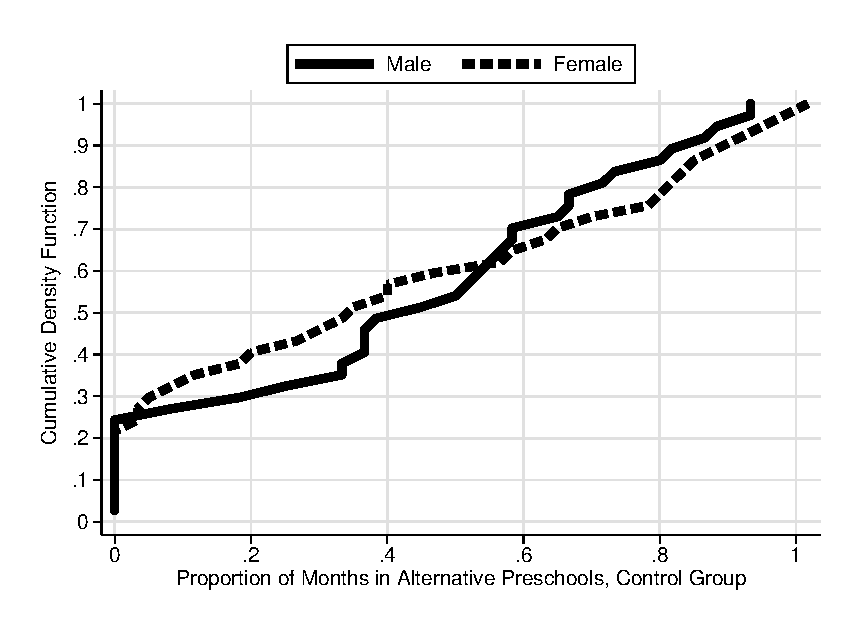
\includegraphics[width=\textwidth]{output/abccare_controlcontamination_boysgirls}
\end{subfigure}%
\begin{subfigure}[h]{0.4\textwidth}
	\centering
	\caption{Socioeconomic Disadvantage by Gender} \label{figure:disadgender}
	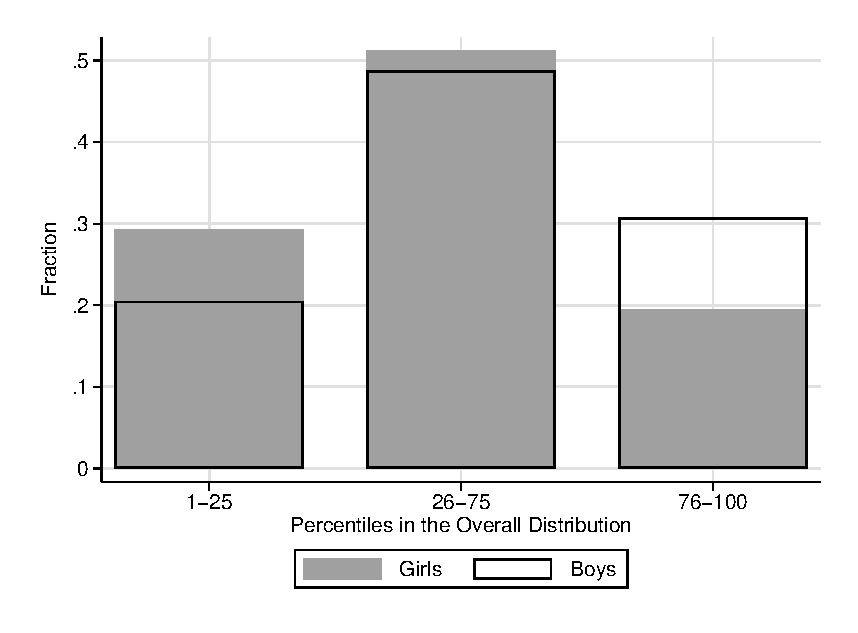
\includegraphics[width=\textwidth]{output/factorbase_girlsboyscompare}
\end{subfigure}
\begin{subfigure}[h]{0.4\textwidth}
	\centering
	\caption{Disadvantage by Take-up of Alternatives, Girls} \label{figure:disadgirls}
	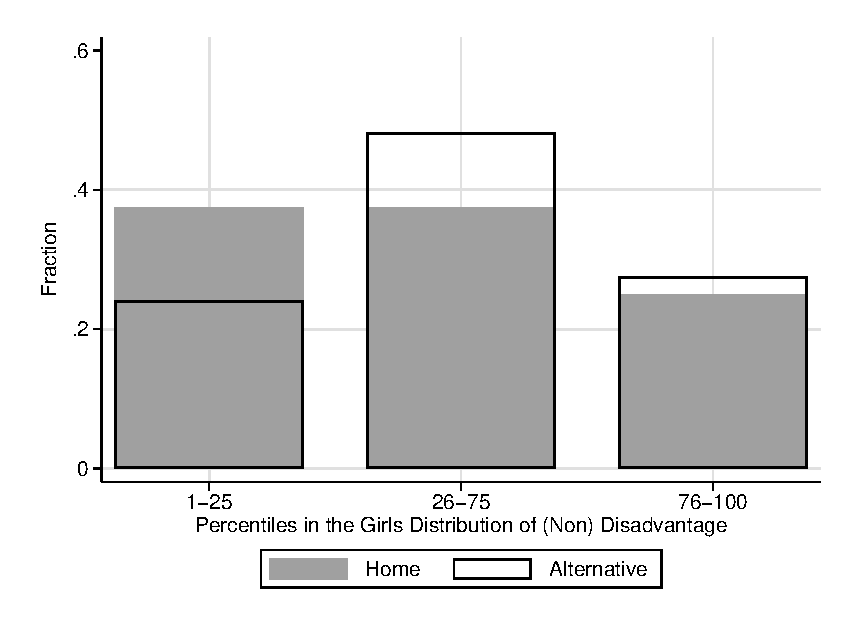
\includegraphics[width=\textwidth]{output/factorbase_wgirlscompare}
\end{subfigure}%
\begin{subfigure}[h]{0.4\textwidth}
	\centering
	\caption{Disadvantage by Take-up of Alternatives, Boys} \label{figure:disadboys}
	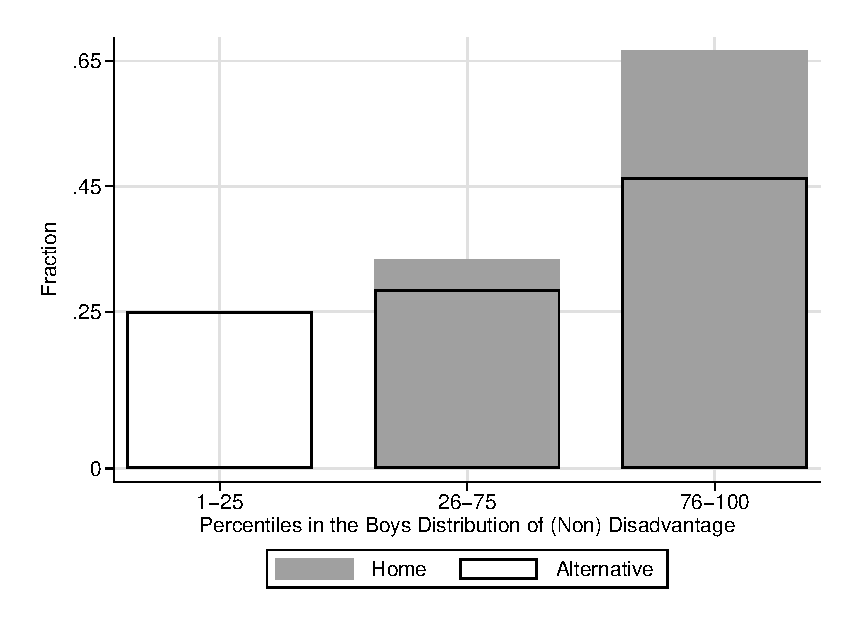
\includegraphics[width=\textwidth]{output/factorbase_wboyscompare}
\end{subfigure}
\footnotesize
\justify
\textbf{Note:} Panel (a) displays the cumulative distribution function of enrollment in alternatives by gender. Panel (b) displays how girls and boys separately fit into the overall (girls and boys pooled) distribution of socioeconomic disadvantage. Panel (c) displays how girls who did not enroll and girls who enrolled in alternatives fit into the overall female distribution of socioeconomic disadvantage. Panel (d) is analogous to Panel (c) for boys. Our measure of socioeconomic disadvantage is a latent of the following variables: Maternal age, education, and IQ, as well as number of siblings and HRI score.
\end{sidewaysfigure}

This difference suggests that boys and girls faced different environments in their control group conditions, especially in their home environments.\footnote{Table~\ref{table:controlsubscharacteristics} summarizes the baseline characteristics by gender and mode of childcare.}\textsuperscript{,}\footnote{An alternative explanation is greater adverse reaction among some boys to being withdrawn from the home environment \citep{Garcia_etal_2019_ECE_IMHJ}. We discuss this possibility at greater length in Section~\ref{sec:conclusion}.} About the same percentage of control-group girls attended alternative formal childcare (73\%) as did control-group boys (76\%). See Figure~\ref{figure:altgender}. No girls who stayed at home had working mothers at baseline while 23\% of the girls who attended alternative formal childcare had mothers working at baseline. For boys, 14\% of those who stayed at home had mothers working at baseline while 29\% of those who attended alternative formal childcare had working mothers.

Girls' families were more resource-constrained compared to their male counterparts. Girls in the control group were raised in a more disadvantaged environment and many likely went to lower-quality preschools. Thus, as documented in Section~\ref{sec:treatment-effects}, they benefited more from participation in ABC/CARE than boys when compared to the next best alternative as perceived by their parents.


To formally test the differences in home-life advantage between control-group girls and boys, we create an index of socioeconomic disadvantage at baseline using mother's age, education, IQ, marital status, and employment, as well as number of children and father's presence at home.\footnote{This index is distinct from HRI.} We assess how girls and boys fit into the overall distribution of this latent measure in the control group. Boys are disproportionately more advantaged than girls (Panel~\ref{figure:disadgender}). In Panels~\ref{figure:disadgirls} and~\ref{figure:disadboys} of Figure~\ref{figure:socdis}, we further assess socioeconomic disadvantage by gender of the child.

Table~\ref{table:disadtests} uses our constructed measure of disadvantage to test the difference in baseline disadvantage across boys and girls. We reject the null hypothesis of a common distribution of socioeconomic disadvantage across girls and boys (at baseline). 

\begin{table}[!htpb]
\begin{threeparttable}
\caption{Gender and Baseline Socioeconomic Disadvantage in the Control Group} \label{table:disadtests}
\centering
\begin{tabularx}{16.5cm}{XcX}
& \begin{tabular}{ccccc}
\toprule
& Males vs. Females & & \mc{2}{c}{Alternatives vs. Home} \\
& & & Males & Females \\
\midrule
 \citet{Rosenbaum_2005_Distribution_JRSS}  & \\
$p$-value & \textbf{0.007} & & \textbf{0.006} & 0.110 \\
\bottomrule
\end{tabular}


% Control, males vs. females: distance between: factor of m_age_base, m_ed_base, m_iq_base, hh_sibs_base, hrabc_index

% Alt. vs home: factor of m_age_base, m_ed_base, m_iq_base, hh_sibs_base, hrabc_index &
\end{tabularx}
\begin{tablenotes}
\footnotesize
\item \textbf{Note:} Row [1] displays an exact, non-parametric $p$-value for the null hypothesis that the control males and control females have the same level of disadvantage. Row [2] displays the same $p$-value for the null  hypothesis that within males, those who attend alternative formal childcare and those who stay at home have the same level of disadvantage. Row [3] is analogous to Row [2] except for females. These tests all use a latent measure of socioeconomic disadvantage (mother's age, education, IQ, marital status, and employment, as well as number of siblings and father's presence at home). Under the null hypotheses, the pairs with the closest distance in disadvantage would be comprised of one male and one female (for the comparison of males vs. females). Rejecting the null implies that the distributions are significantly different. Statistics significant at the $0.10$ level are bolded.
\end{tablenotes}
\end{threeparttable}
\end{table}

Parents of more advantaged girls in the control group are more likely to send their daughters to alternative preschools. Parents of more advantaged boys in the control group are more likely to keep their sons at home. Thus, boys benefited more from treatment when compared to attending alternative formal childcare as opposed to staying at home where they faced better environments than girls. The opposite pattern holds for girls, although the differences between the treatment effects by mode of alternative childcare are smaller for girls than for boys. 

As shown in Section~\ref{sec:treatment-effects}, the childcare supplied by ABC/CARE increases maternal employment and family income in childhood. This effect is especially pronounced for the mothers of girls. Differentially higher employment of mothers induced by the program led to larger treatment effects for income for families of girls as a result of the childcare afforded mothers. HOME scores are also differentially enhanced for girls.

More fathers are present for boys. At baseline, this leads to more family resources for boys. Family income is higher for boys than girls after treatment despite the differential treatment effect in employment for the mothers of girls. While boys benefit from the greater presence of the father, there is no program-induced treatment effect attracting fathers to stay the home.


